% Figure from MATH 556 notes, section 4. Compile with the notes preamble.
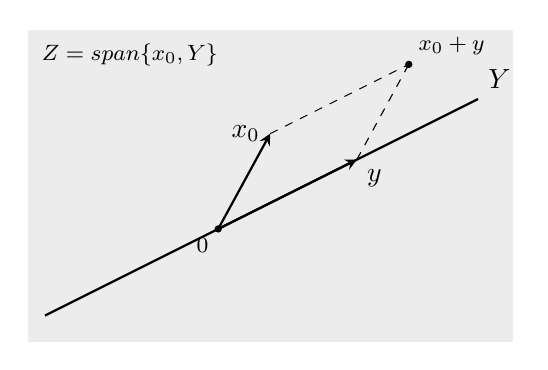
\begin{tikzpicture}[scale=1.1, >=stealth]
    \fill[gray!15] (-2.2,-1.3) rectangle (3.4,2.3);
    \node[font=\footnotesize, anchor=north west] at (-2.15,2.25) {$Z = \operatorname{span}\{x_0, Y\}$};
    \draw[thick] (-2.0,-1.0) -- (3.0,1.5) node[above right] {$Y$};
    \draw[->, thick] (0,0) -- (0.6,1.1) node[left] {$x_0$};
    \draw[->, thick] (0,0) -- (1.6,0.8) node[below right] {$y$};
    \draw[dashed] (1.6,0.8) -- (2.2,1.9);
    \draw[dashed] (0.6,1.1) -- (2.2,1.9);
    \fill (2.2,1.9) circle (1.2pt) node[above right, font=\footnotesize] {$x_0 + y$};
    \fill (0,0) circle (1.2pt) node[below left, font=\footnotesize] {$0$};
\end{tikzpicture}
